\section{Classification}

After every frame in a sample has been through the modelfitting process, we can analyse the sequence as a whole
and produce a series of numbers which describe the subject's gait.
If we are successful, this series of numbers will be unique to each subject and can be used as the basis for classifying any new samples.


\subsection{Extracting a gait cycle}
\label{ExtractingGaitCycle}

Before we can perform any kind of analysis on a sample we need to identify and extract one gait cycle.
This is important because we will be comparing different samples which might begin at different times during the subjects' gait cycle.

\begin{figure}[tb]
	\centering
	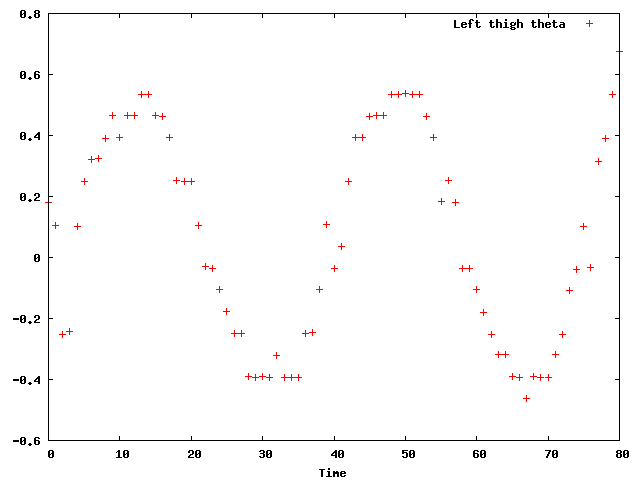
\includegraphics[width=\textwidth]{curvefitting.png}
	\caption{The change in $\theta_1$ over time for Sample 81.}
	\label{CurveFitting1}
\end{figure}

Figure \ref{CurveFitting1} shows a typical plot of the change in the value of $\theta_1$ over time.
The graph resembles a sinosoid which we intuitavely know to be correct - when we walk our thighs swing forwards and backwards like a pendulum.
A gait cycle is usually defined as beginning and ending with heel strikes of the same foot \cite{PIEEE}, which in Figure \ref{CurveFitting1} would be two subsequent maximums of the sinosoid.
We however are going to begin our gait cycle when the thigh crosses the vertical, ie. when $\theta = 0$.

We can find this point where the thigh crosses the vertical by fitting a function $f_1(t)$ to our data points and finding where $f_1(t) = 0$.
The function we use is shown in Equation \ref{eqn:CurveFitting}:

\begin{equation}
	f_1(t) = d + a \sin\left(\frac{2 \pi t}{\xi} + \phi\right)
	\label{eqn:CurveFitting}
\end{equation}

The DC offset, $d$, and amplitude, $a$, were found to be fairly similar for all subjects, so were kept fixed at $d = 0.05$ and $a = 0.55$.
Least squares regression was used to find the values for $\xi$, the period of the gait cycle, and $\phi$, the phase offset.

\begin{figure}[tb]
	\centering
	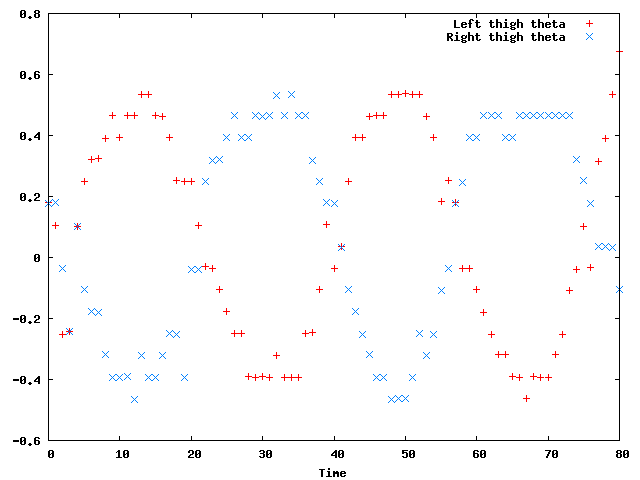
\includegraphics[width=\textwidth]{curvefitting2.png}
	\caption{The change in $\theta_1$ and $\theta_2$ over time for Sample 81.
		The two parameters are $90^\circ$ out of phase.}
	\label{CurveFitting2}
\end{figure}

Equation \ref{eqn:CurveFitting} above describes the general motion of only one of the thighs.
We can increase accuracy by including the motion of the other thigh as well.
We make use of the observation that the motion of the two thighs are $90^\circ$ out of phase (see Figure \ref{CurveFitting2}):

\begin{equation}
	f_2(t) = d + a \sin\left(\frac{2 \pi t}{\xi} + \phi + \pi\right)
	\label{eqn:CurveFitting2}
\end{equation}

The implementation used for our least squares fitting is similar to that in Listing \ref{leastsquarescode}, however instead of looking over a four-dimensional parameter space we are only interested in $\xi$ and $\phi$.
The ranges used for these variables are $\xi = [30, 40]$ and $\phi = [0, 2\pi]$.
The assumption that the period of one gait cycle lies in this range $[30, 40]$ was arrived at by observation of the typical gait cycles in our database.

The energy function used to determine the suitability of each set of parameters is worth mentioning as it has to take into account two curves and two sets of data.
It is shown in Listing \ref{curvefittingenergy}.
This function is used in a similar way to $modelEnergy$ in Listing \ref{leastsquarescode}.

\begin{lstlisting}[firstnumber=1,language=c,morekeywords={step,function,foreach,in},frame=single,mathescape=true,caption={Energy function pseudo-code},label={curvefittingenergy},float=[tb]]
function energy($\xi$, $\phi$)
	$d = 0.05$
	$a = 0.55$
	
	$energy = 0$
	foreach $t$
		$expected_{left} = d + a \sin(\frac{2 \pi t}{\xi} + \phi)$
		$expected_{right} = d + a \sin(\frac{2 \pi t}{\xi} + \phi + \pi)$
		$actual_{left}$ = $\theta_1$[$t$]
		$actual_{right}$ = $\theta_2$[$t$]
		
		$energy$ += $(expected_{left} - actual_{left})^2$
		$energy$ += $(expected_{right} - actual_{right})^2$
	
	return $energy$
\end{lstlisting}

Once we have obtained values for $\xi$ and $\phi$ we can find the time $z$ of each zero-crossing like so:

\begin{equation}
	z_i = \frac{\xi \sin^{-1}\left(-\frac{d}{a} - \phi\right)}{2\pi} + i\pi
\end{equation}


\subsection{Discrete fourier transforms}

Now that we can extract a gait cycle from each sample we need to apply the DFT (Discrete Fourier Transform) to them to obtain information about the frequency components of the subject's gait.
These frequency components can hopefully be used to form an identifying signature for the subject.

The DFT is defined by Equation \ref{eqn:DFT}.
A series $x$ of $N$ complex numbers is transformed into another series $X$ of $N$ complex numbers.
The number $X_i$ represents the $i^\text{th}$ multiple of the fundamental frequency (which is defined as $\frac{1}{N}$).

\begin{equation}
	X_i = \sum_{k=0}^{N-1} x_k e^{-\frac{2 \pi i}{N} i k} \quad \quad i = 0, \dots, N-1
	\label{eqn:DFT}
\end{equation}

Our input data to the DFT is purely real valued, so the output will obey the symmetry:

\begin{equation}
	X_i = X_{N-k}^*
\end{equation}

We can therefore disregard the second half of the output, as it will contain the same information as the first half.

The FFTW library \cite{FFTW} was used in the Modelfitter application to calculate the DFT.
Some typical results are shown in Figure \ref{FFTResults}.

\begin{figure}[tb]
	\centering
	\subfloat[Magnitude]{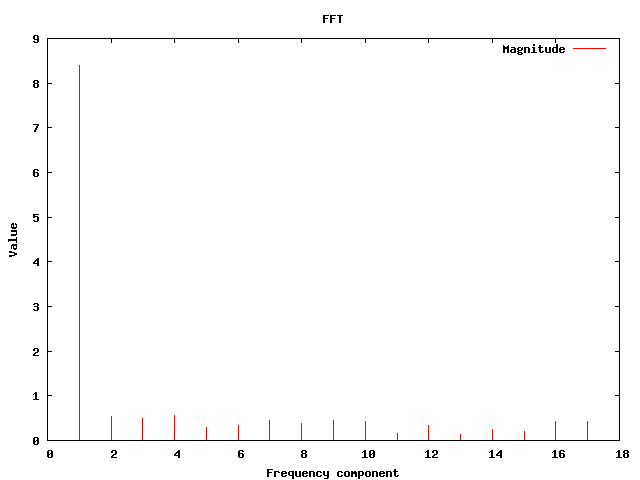
\includegraphics[width=5cm]{dft-leftthightheta-magnitude.png}}
	\quad
	\subfloat[Phase]{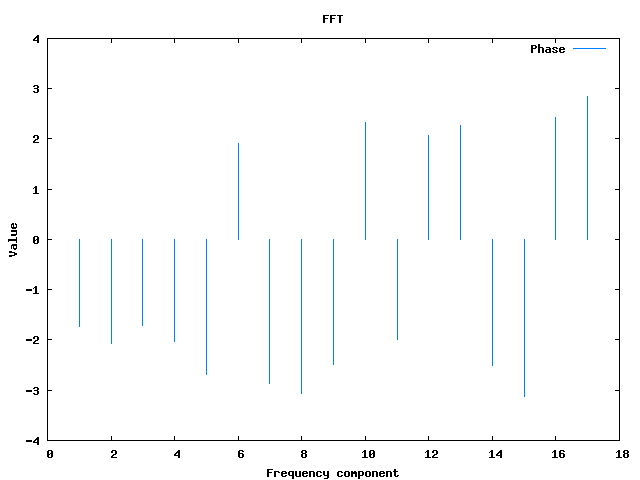
\includegraphics[width=5cm]{dft-leftthightheta-phase.png}}
	\caption{Results of taking the DFT of $\theta_1$ from one gait cycle of Sample 81.}
	\label{FFTResults}
\end{figure}


\subsection{Classification methods}
\label{ClassificationMethods}

To correctly classify a new sample, we need some way of comparing it to the other samples already in the database.
The k-nearest neighbour algorithm with $k=1$ was chosen as it is simple to implement while providing good results.

A distance function $d(a,b)$ was created to compare and evaluate the difference between two samples $a$ and $b$.
Each sample consists of $\frac{N}{2}$ complex numbers - the output of the DFT.

Several different implementations for this function were tested.
Details of each are given below, and quantitative comparisons of their performance can be found in section \ref{Results:Classification}.

\begin{enumerate}
	\item \textbf{Magnitude}.
		The magnitudes of each frequency component are compared.
		\begin{equation}
			d(a, b) = \sum_{i=1}^{N/2} \left( \left|a_i\right| - \left|b_i\right| \right)^2
		\end{equation}
	
	\item \textbf{Magnitude-weighted phase}.
		Phase information is also taken into account, but it is weighted by the magnitude to ensure that
		the very low magnitude frequency components do not overly influence the result.
		\begin{equation}
			d(a, b) = \sum_{i=1}^{N/2} \left( \left|a_i\right| \arg a_i - \left|b_i\right| \arg b_i \right)^2
		\end{equation}

	\item \textbf{Euclidean distance in complex plane}.
		A problem with comparing the phase directly is that the difference between two phase values $+\frac{5}{6}\pi$ and $-\frac{5}{6}\pi$ will
		equal $\frac{10}{6}\pi$ when actually, due to the modulo nature of phase, it should equal only $\frac{2}{6}$.
		In an attempt to solve this we compare the real and imaginary parts directly.
		\begin{equation}
			d(a, b) = \sum_{i=1}^{N/2} \left( \Re{a_i} - \Re{b_i} \right)^2 + \left( \Im{a_i} - \Im{b_i} \right)^2
		\end{equation}
	
	\item \textbf{Polar distance}.
		This is another measure that can be used to calculate the distance between two points on the complex plane.
		\begin{equation}
			d(a, b) = \sum_{i=1}^{N/2} \left|a_i\right|^2 + \left|b_i\right|^2 - 2 \left|a_i\right| \left|b_i\right|^2 \cos\left(\arg a_i - \arg b_i\right)
		\end{equation}
	
	\item \textbf{Mean normalization}.
		It may boost performance to normalize each of the samples so the mean of their frequency components is zero.
		This can be done by first finding the mean:
		\begin{align}
			\mu_a &= \frac{2}{N} \sum_{i=1}^{N/2} a_i \\
			\mu_b &= \frac{2}{N} \sum_{i=1}^{N/2} b_i
		\end{align}
		and then subtracting this mean from each of the frequency components:
		\begin{align}
			a_i' &= a_i - \mu_a \\
			b_i' &= b_i - \mu_b
		\end{align}
		These new values $a_i'$ and $b_i'$ can then be used in the above difference functions in place of $a_i$ and $b_i$.
	
	\item \textbf{Exclude first component}.
		Note that we take the first component to mean the first multiple of the fundamental frequency and assume that any DC offset has already been removed
		by mean normalization.
		As can be seen in Figure \ref{FFTResults} the magnitude of the first frequency component is very large.
		This is the case for every sample, so perhaps better classification can be performed by ignoring this first component.
		This can be done by changing the sum on each of the previous equations to $\sum_{i=2}^{N/2}$.
\end{enumerate}


\subsection{Additional classification metrics}

In \cite{StrideCadence} BenAbdelkader et al.\ show how four static parameters - namely the body height, torso length, leg length and step length - can be extracted from a video sequence and used to identify a subject.
We already extract the body height in section \ref{LocatingCenter}, but in our model the torso length and leg length are both assumed to be half of the body height.

The step length can be calculated from the gait period as determined in \ref{ExtractingGaitCycle}, but this is not necessairly a good identifying measure.
In preliminary analysis of our data set it was noted that, while the period of one gait cycle does vary between subjects, the overall spread and distance between classes is very small.

